\documentclass[]{beamer}
% Class options include: notes, notesonly, handout, trans,
%                        hidesubsections, shadesubsections,
%                        inrow, blue, red, grey, brown

% Theme for beamer presentation.
\usepackage{beamerthemesplit} 
% Other themes include: beamerthemebars, beamerthemelined, 
%                       beamerthemetree, beamerthemetreebars  

\title{National Wage Setting: Interesting Results}
\author{Isaac Liu}
\date{\today}

\usepackage{graphicx} % http://ctan.org/pkg/graphicx
\usepackage{amsmath}
\usepackage{geometry}
\usepackage{amsfonts}
\usepackage[english]{babel}
\usepackage{amssymb}
\usepackage{graphicx}
\usepackage{float}
\usepackage{hyperref}
\usepackage{multirow}
\usepackage{pdflscape}
\usepackage{caption}
\usepackage{pdflscape}
\usepackage{outlines}
\usepackage{subcaption}

\usepackage{tabularx, booktabs}

\usepackage{standalone}

\usepackage[autostyle, english = american]{csquotes}
\MakeOuterQuote{"}

\usepackage{comment}

\hypersetup{
    colorlinks=true,
    linkcolor=blue,
    filecolor=magenta,      
    urlcolor=cyan,
}

\begin{document}

\begin{frame}
    \frametitle{Commitment Institutions and Electoral and Political Instability}
    \begin{itemize}
        \item Isaac Liu
    \end{itemize}
\end{frame}

\begin{frame}
\frametitle{Do the commitment institutions of central bank independence and fixed exchange rates affect electoral and political instability?}
\begin{itemize}
\item Net Welfare Benefits
\begin{itemize}
\item Inflation Time Inconsistency
\item Political efficacy, access to capital
\item Economic Voting, Increased Stability
\end{itemize}
\item Political Business Cycles
\begin{itemize}
\item Inability to manipulate economy or satisfy partisans
\item Monetary (perhaps fiscal) policy
\item Economic voting, Decreased Stability
\end{itemize}
\end{itemize}

\includegraphics{img0000.png}
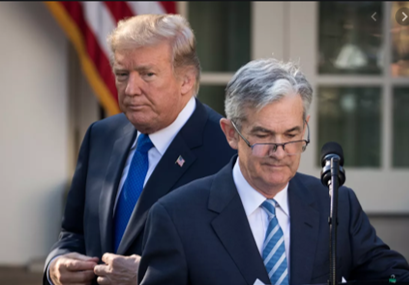
\includegraphics{img0001.png}
\end{frame}


\begin{frame}
\frametitle{Literature}
\begin{itemize}
\item Bernhard and Leblang (2002)
\begin{itemize}
\item OLS, 16 parliamentary democracies since 1970s
\item CBI increases cabinet duration by 3mos, Fixed rates by 5mos
\end{itemize}
\item Clark, Golder, and Poast (2013)
\begin{itemize}
\item Survival Analysis, 19 OECD countries since 1970s
\item Both institutions increase leader survival but only after 7y in office
\end{itemize}
\item Contribution:
\begin{itemize}
\item Far larger dataset including non/semi-democracies
\item More consideration of endogeneity: choice of institutions based on stability consideration, de jure independence
\item Political, not just electoral stability (coups, civil wars, etc), consideration for specific governmental positions
\end{itemize}
\end{itemize}
\end{frame}


\begin{frame}
\frametitle{Data}
\begin{itemize}
\item Panel of 192 countries, 1970-2016
\item Varieties of Democracy
\begin{itemize}
\item V2elturnhos, v2eltturnhog, v2eltvrig
\item 0 for same individual, 1 for same party or coalition, 2 for new party \& ind.
\item WGI Political Violence (neg = unstable)
\item Instability Event- coup, civil war, internal conflict
\end{itemize}
\item Garriga (Cukierman, Webb, Neyapti)- de jure CBI
\item Dreher et al.- Irregular turnover of governor- de facto CBI
\item Reinhart, Rogoff Exchange Rates: 16 categories (higher = float)
\end{itemize}
\end{frame}


\begin{frame}
\frametitle{Results}
\begin{itemize}
\item FEs, clustered SEs
\item De Jure CBI and more instability: PBCs
\item Less De Facto CBI (high irregular turnover) and more lower chamber turnover
\item Floating rate and HOS turnover
\item Welfare Benefits of De Facto CBI, Fixed Rates?
\end{itemize}
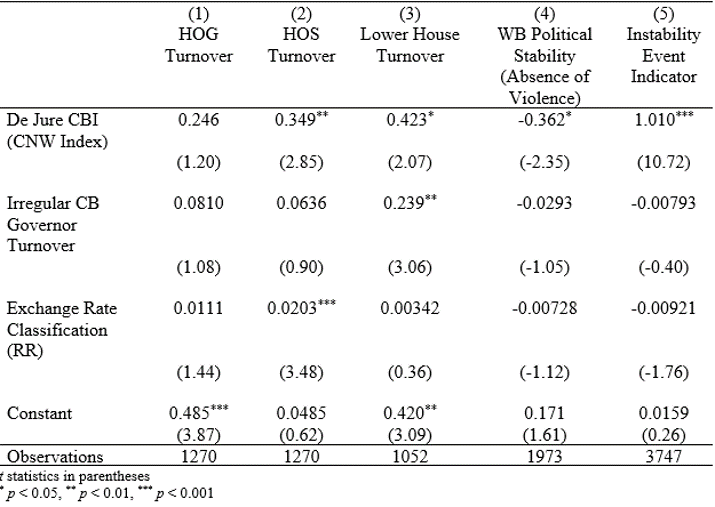
\includegraphics{img0002.png}
\end{frame}


\begin{frame}
\frametitle{Ordered Logit (Mean Marginal Effects)}
\begin{itemize}
\item Nothing changes in terms of significance, except for fixed Erates and HOG
\item xtologit; random effects
\end{itemize}
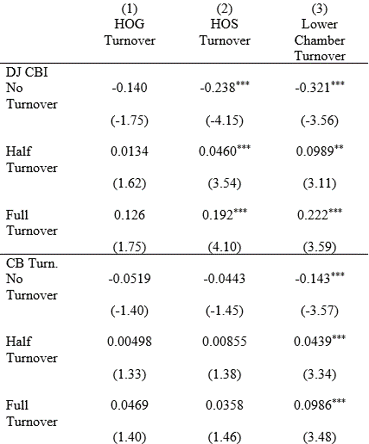
\includegraphics{img0003.png}
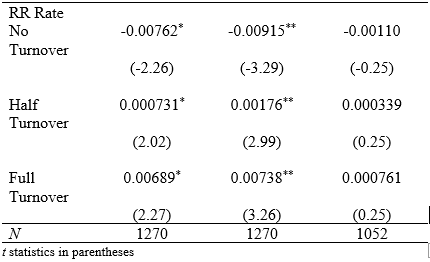
\includegraphics{img0004.png}
\end{frame}


\begin{frame}
\frametitle{Panel Logit (binary instability event variable) Mean Marginal Effects}
\begin{itemize}
\item Fixed effects
\item More evidence that de jure CBI increases political instability
\item Fixed exchange rate (low RR rate) increases pol. instability, but very small effect size
\end{itemize}
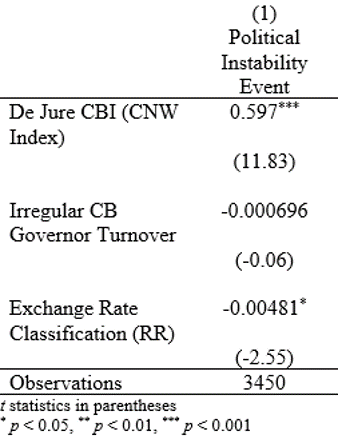
\includegraphics{img0005.png}
\end{frame}


\begin{frame}
\frametitle{IV1: Tertiary Ed Enrollment (CBI),Aggregate GDP (Fixed Rate)}
\begin{itemize}
\item Good first stages
\item Poor exclusion restrictions for political stability, better ones for electoral stability/turnover
\item De jure CBI now increases lower chamber turnover, but no longer HOS
\item Unclear sign for fixed rates (last two cols)
\item De facto CBI omitted, insignificant
\end{itemize}
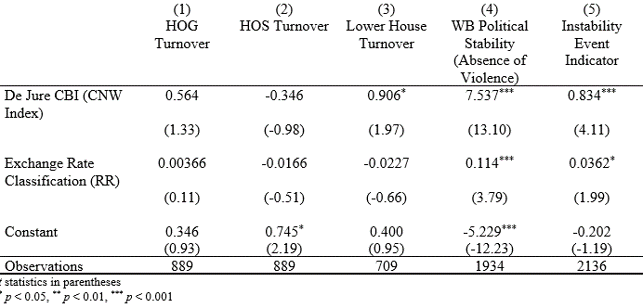
\includegraphics{img0006.png}
\end{frame}


\begin{frame}
\frametitle{IV2: Population Share Social Science/Business Grads (CBI), Agg GDP (Fixed Rates)}
\begin{itemize}
\item Better Exclusion Restriction
\item Very limited data but strong result for de jure CBI and political instability
\end{itemize}
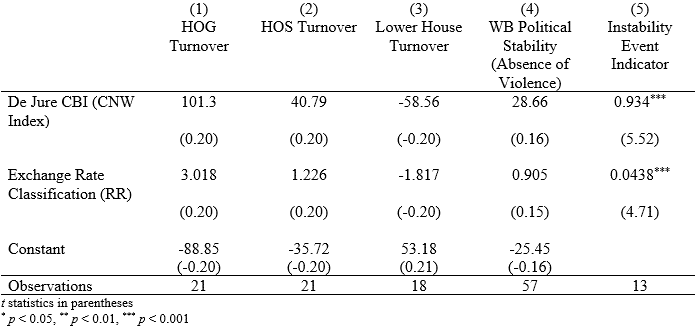
\includegraphics{img0007.png}
\end{frame}


\begin{frame}
\frametitle{Just Aggregate GDP for Fixed Rates}
\begin{itemize}
\item Clearer case for fixed rates decreasing pol and electoral stability (PBC)
\item Note on exclusion restriction: still an imperfect case
\begin{itemize}
\item Agg GDP proxies for economy size (optimum currency area)
\item Arguably not as connected to GDP per capita to stability
\end{itemize}
\item Result for LH sensitive to dataset
\end{itemize}
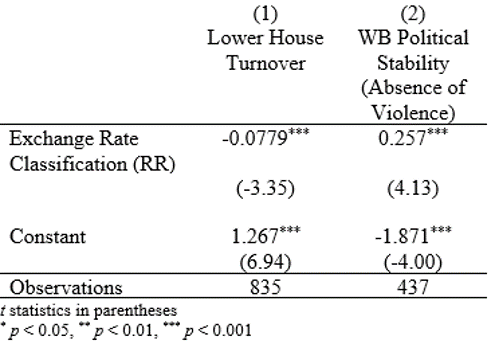
\includegraphics{img0008.png}
\end{frame}


\begin{frame}
\frametitle{Table of Lags}
\begin{itemize}
\item Irregular central bank turnover instantaneously associated with lower chamber election turnover
\item T-3 sees strongest de jure CBI political instability impact
\item T-6, T-8 de jure CBI increases pol instability. T-8 reduces HOG turnover (electoral instability) (similar to Clark, Golder, and Poast).
\item Fixed rates increase instability in the same T-6 and up range
\item Little significance for de facto CBI/governor turnover
\end{itemize}
\end{frame}


\begin{frame}
\frametitle{Summary}
\begin{itemize}
\item De jure CBI generally decreases (esp. pol) stability, suggesting limits on PBCs
\item Sign unclear for governor turnover/de facto CBI
\item Fixed exchange rates also increase electoral stability, but decrease political stability in FE \& XTLogit models
\item In IV and lag specifications fixed rates decrease all stability
\item Commitment institutions politically costly, at odds with literature
\item Robust results
\begin{itemize}
\item Not covered: capital controls/openness don’t matter, binary independent variables somewhat reduce effect sizes, interactions with democracy do not matter, institutional controls for federalism and corporatism do not affect signs or cause large changes in effects
\end{itemize}
\end{itemize}
\end{frame}


\begin{frame}
\frametitle{Questions/future directions}
\begin{itemize}
\item Diverging predictions for Head of Government, Head of State, Lower House Turnover
\begin{itemize}
\item HOS and Lower House seem to have strongest relationships
\end{itemize}
\item Recode/reverse exchange rate variable
\item Endogenous elections
\item Exchange rate classification as categorical variable, not continuous
\item Dynamic panel (A-Bond)?
\item Ordinal logit regression with IV (different procedure)
\item Ordinal logit with lags
\end{itemize}
\end{frame}


\begin{frame}
\frametitle{Additional Results/Checks}
\end{frame}


\begin{frame}
\frametitle{HOS = HOG?}
\begin{itemize}
\item V2exhoshog is an indicator for whether HOS and HOG are the same person
\item De jure CBI increases HOS turnover somewhat more when they are not the same person ???
\item Weaker effect when they are
\item Fixed erates reduce turnover in when they are the same person
\end{itemize}
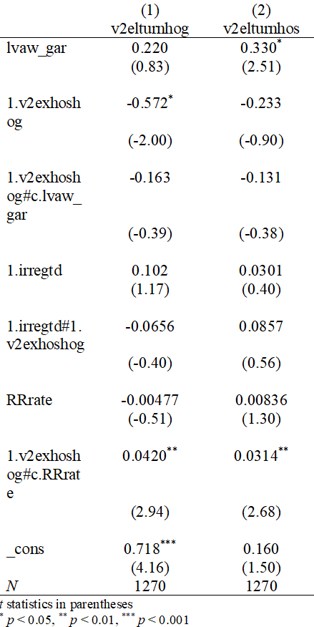
\includegraphics{img0009.png}
\end{frame}


\begin{frame}
\frametitle{Binary Dependent Variable (xtlogit)}
\begin{itemize}
\item Two codings, similar results
\item Fixed effects
\item Floating (versus fixed) rate now also increases WB political instability index
\end{itemize}
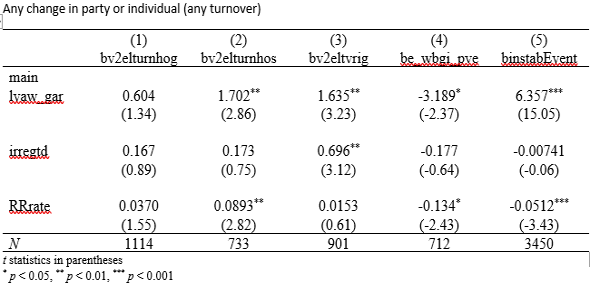
\includegraphics{img0010.png}
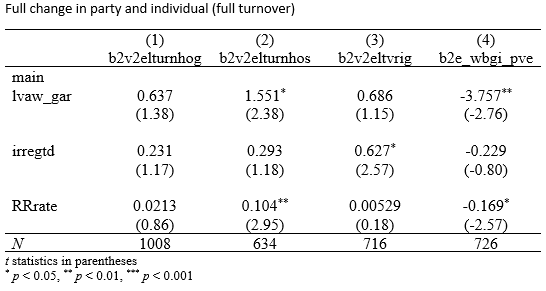
\includegraphics{img0011.png}
\end{frame}


\begin{frame}
\frametitle{Controls}
\begin{itemize}
\item Regional government exists and has autonomy and authority, checks and balances/horizontal accountability
\item Not strictly necessary
\begin{itemize}
\item FEs
\item No sign flips
\end{itemize}
\item Omitted: Corporatism
\item Collinearity?
\end{itemize}
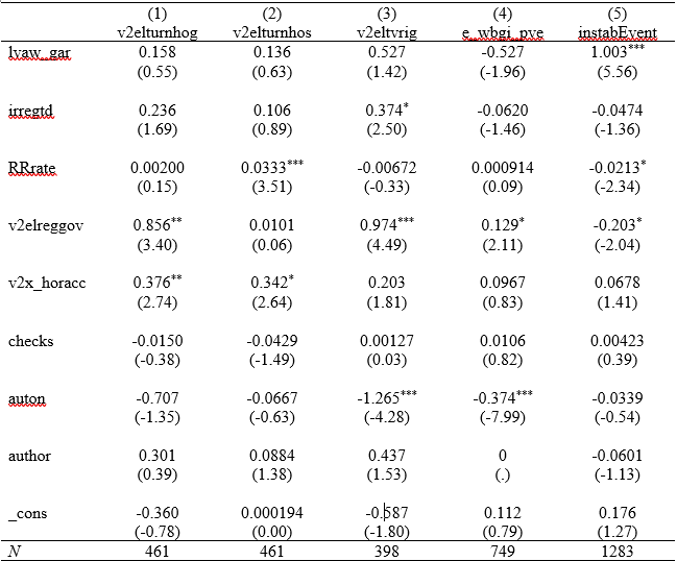
\includegraphics{img0012.png}
\end{frame}


\begin{frame}
\frametitle{Democracy/Nondemocracy}
\begin{itemize}
\item High polity on the left, low polity on the right
\item De facto CBI (less irregular turnover) means less lower chamber turnover in democracies but reverse in autocracies. Rule of law?
\end{itemize}
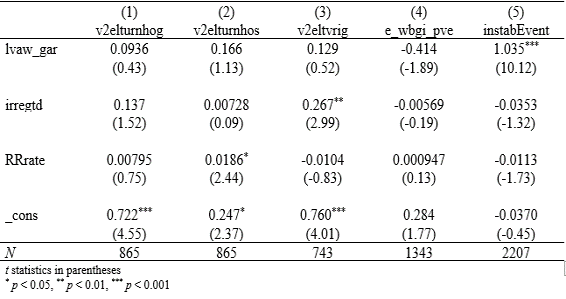
\includegraphics{img0013.png}
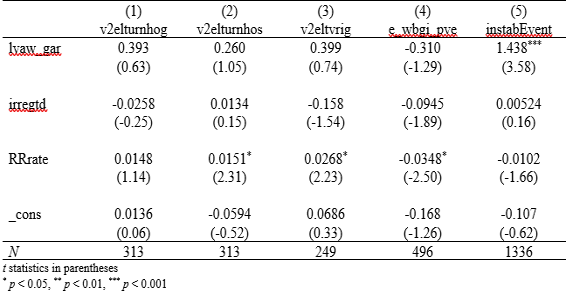
\includegraphics{img0014.png}
\end{frame}
